%%%%%%%%%%%%%%%%%%%%%%%%%%%%%%%%%%%%%%%%%
% Stylish Article
% LaTeX Template
% Version 2.2 (2020-10-22)
%
% This template has been downloaded from:
% http://www.LaTeXTemplates.com
%
% Original author:
% Mathias Legrand (legrand.mathias@gmail.com)
% With extensive modifications by:
% Vel (vel@latextemplates.com)
%
% License:
% CC BY-NC-SA 3.0 (http://creativecommons.org/licenses/by-nc-sa/3.0/)
%
%%%%%%%%%%%%%%%%%%%%%%%%%%%%%%%%%%%%%%%%%

%----------------------------------------------------------------------------------------
%	PACKAGES AND OTHER DOCUMENT CONFIGURATIONS
%----------------------------------------------------------------------------------------

\documentclass[fleqn,10pt]{SelfArx} % Document font size and equations flushed left

\usepackage[english]{babel} % Specify a different language here - english by default
\usepackage{pgfgantt}

\usepackage{lipsum} % Required to insert dummy text. To be removed otherwise

%----------------------------------------------------------------------------------------
%	COLUMNS
%----------------------------------------------------------------------------------------

\setlength{\columnsep}{0.55cm} % Distance between the two columns of text
\setlength{\fboxrule}{0.75pt} % Width of the border around the abstract

%----------------------------------------------------------------------------------------
%	COLORS
%----------------------------------------------------------------------------------------

\definecolor{color1}{RGB}{0,0,90} % Color of the article title and sections
\definecolor{color2}{RGB}{0,20,20} % Color of the boxes behind the abstract and headings

%----------------------------------------------------------------------------------------
%	HYPERLINKS
%----------------------------------------------------------------------------------------

\usepackage{hyperref} % Required for hyperlinks

\usepackage{float}
\usepackage{makecell}
\hypersetup{
	hidelinks,
	colorlinks,
	breaklinks=true,
	urlcolor=color2,
	citecolor=color1,
	linkcolor=color1,
	bookmarksopen=false,
	pdftitle={Title},
	pdfauthor={Author},
}
\usepackage{multicol}

%----------------------------------------------------------------------------------------
%	ARTICLE INFORMATION
%----------------------------------------------------------------------------------------

\JournalInfo{Laboratory of biological data mining} % Journal information
\Archive{Project report} % Additional notes (e.g. copyright, DOI, review/research article)

\PaperTitle{Identification and validation of a vitamin D-related prognostic signature in colorectal cancer} % Article title

\Authors{Diego Barquero Morera\textsuperscript{1}, Giacomo Fantoni\textsuperscript{2}, Gaia Faggin\textsuperscript{3}, Leonardo Golinelli\textsuperscript{4}} % Authors
\affiliation{\textsuperscript{1}\textit{diego.barqueromorera@studenti.unitn.it}} % Author affiliation
\affiliation{\textsuperscript{2}\textit{giacomo.fantoni@studenti.unitn.it}} % Author affiliation
\affiliation{\textsuperscript{3}\textit{gaia.faggin@studenti.unitn.it}} % Author affiliation
\affiliation{\textsuperscript{4}\textit{leonardo.golinelli@studenti.unitn.it}} % Author affiliation

\Keywords{} % Keywords - if you don't want any simply remove all the text between the curly brackets
\newcommand{\keywordname}{Keywords} % Defines the keywords heading name

%----------------------------------------------------------------------------------------
%	ABSTRACT
%----------------------------------------------------------------------------------------

\Abstract{}
%----------------------------------------------------------------------------------------

\begin{document}

\maketitle % Output the title and abstract box

\tableofcontents % Output the contents section

\thispagestyle{empty} % Removes page numbering from the first page

%----------------------------------------------------------------------------------------
%	ARTICLE CONTENTS
%----------------------------------------------------------------------------------------

\section{Introduction}
Colorectal cancer (CRC) is the third most common malignant tumor worldwide and is the second one in cancer-related deaths [1]. In spite of improvements in the management and treatments of patients with CRC in the last two decades, no satisfactory therapy exists when the surgery is not curative. The poor prognosis and the increasing incidence of CRC have provided strong motivation to construct a predictive model in CRC patients, which will benefit personalized treatment in clinical management [2]. There are lot of epidemiological and preclinical studies that indicate a beneficial effect of vitamin D on CRC incidence and mortality [3] [4]. Vitamin D is a fat soluble vitamin and many genes are related to its metabolism and action [5]. It can be obtained from diet or the endogenous synthesis in the epidermis under sunlight exposure [6]. It has been demonstrated that vitamin D benefits clinical outcome and improves the long-term survival of CRC patients [7]. Moreover, circulating vitamin D may be a CRC biomarker and its deficiency is related to the high incidence of CRC [8]. A better survival outcome in CRC is associated with higher prediagnostic or postdiagnostic serum 25-hydroxyvitamin D concentrations [9]. The most active vitamin D metabolite (1$\alpha$,25-dihydroxyvitamin D3) inhibits the proliferation and promotes the differentiation of cultured colon carcinoma cells by mechanisms that include cell cycle arrest at G0/G1 phase, blockade of the Wnt/$\beta$-catenin pathway and induction of Ecadherin and other epithelial proteins [3] [10] [11]. Lots of genes related to vitamin D metabolism and action play an essential role in tumors. For example, CYP24A1 an important vitamin D-related gene, is up-regulated in CRC patient and nominated as a promising biomarker [12]. Vitamin D and its related genes are correlated with the homeostasis of the intestinal epithelium and regulate immune cells [13].

The objective of this project was to find a way to make prognosis and stratify patients suffering from colorectal cancer by means of their transcriptomic profiles. In particular we focused on the gene signature of vitamin D as a prognostic marker, by leveraging the always increasing gene expression data publicly available. The final goal was to identify colorectal cancer survival markers related with vitamin D effects, as well as any pathways involved.


\section{Material and methods}

	\subsection{Data preprocessing}
	To achieve a better statistical significance, a high number of samples was originally collected from different available public datasets on gene expression in CRC. These were downloaded from the databases Gene Expression Omnibus (GEO) [cite] and The Cancer Genome Atlas (TCGA) [cite]. In total, 21 datasets from GEO and 1 from TCGA were obtained, and their metadata manually curated and standardized (table 1). It is worth noting that only the dataset GSE157982 had the gene signature of Vitamin D in CRC, necessary for its further analysis.

	\begin{table*}[ht]
		\centering
		\begin{tabular}{cccc}
			\hline
			Dataset name & Sample description & Number of samples\\
			\hline
			E-MTAB-6698	& healthy and tumor colorectal samples	&1566\\
			GSE157982	&baseline and vit. D-treated CRC rectal samples	&98\\
			GSE38832	&tumor colorectal samples	&122\\
			TCGA-COAD	&tumor colorectal samples	&438\\
			GSE14333	&tumor colorectal samples	&290\\
			GSE17536	&tumor colorectal samples	&177\\
			GSE31595	&tumor colorectal samples	&37	\\
			GSE33113	&tumor colorectal samples	&96	\\
			GSE38832	&tumor colorectal samples	&122\\
			GSE39084	&tumor colorectal samples	&70	\\
			GSE39582	&tumor colorectal samples	&585\\
			GSE103479	&tumor colorectal samples	&156\\
			GSE17537	&tumor colorectal samples	&55	\\
			\hline
		\end{tabular}
		\caption{Starting datasets}
		\label{tab:datasets}
	\end{table*}

		\subsubsection{Sample splitting and filtering}
		In order to filter the samples having all the data necessary for the downstream analyses, they were split in 6 sets according to their available clinical data. Metadata to be considered was, for instance, survival time and tumor stage. After this operation, 2676 samples were retained out of the starting 3072 ($87.11\%$), divided as in table \ref{tab:samples_split}.

		\begin{table}[H]
			\centering
			\begin{tabular}{cc}
				\hline
				Set usage & $n^\circ$ of samples\\
				COX fitting & $388$\\
				KM curve & $157$\\
				Vitamine D low & $49$\\
				Vitamine D high & $49$\\
				Stage low & $1120$\\
				Stage high & $908$\\
				\hline
			\end{tabular}
			\caption{Split samples}
			\label{tab:samples_split}
		\end{table}

		\subsubsection{Dataset normalization}

			\paragraph{fRMA}

			\paragraph{Bootstrap}

	\subsection{Differentially expressed genes}
	After having removed the batch effect and having obtained all the necessary datasets we used them two set of differentially expressed genes, from here \emph{DEGs}.
	The first step contains DEGs found in different stages of cancer and the second the vitamin-D gene signature.

		\subsubsection{DEG between stage of cancer}
		For each of the $10$ subset of the used samples a LIMMA analysis was performed.
		The resulting gene lists have been sorted in increasing order by p-value.
		We aggregated the resulting list using Borda count, so to obtain a ranking for each of the $temp$ genes.
		This ranking will be used to see if the genes we found downstream are responsible for differentiating between cancer stages.

		\subsubsection{Vitamin D gene signature}
		In order to obtain the list of differentially expressed genes for the vitamin D signature, the state-of-the-art R package “Deseq2” was used on the vitamin D dataset, which contains counts of RNA-seq expression data from rectal biopsies of CRC patients pre-and post- vitamin D supplementation. Transcript IDs were converted to Gene Symbols through “BioMart”. For some of the transcripts, a Gene Symbol was not found. The statistically relevant genes were then selected using the adjusted p-value automatically computed by the Deseq2 package. DEGs were then manually expanded using the protein-protein interaction network database STRING.
Enrichment analysis was performed on the original list using the web interface EnrichR.


	\subsection{Survival analysis}
	The survival analysis has been used to determine if both sets of DEGs we found upstream are responsible for a change in the probability of survival.
	This analysis has been performed in two steps.
	The first uses a cox proportional-hazards model and the second involves building the Kaplan-Meier curves for the significative gene found by cox on a different dataset.

		\subsubsection{Cox proportional-hazards model}
		Cox-proportional-hazards model is used to determine for each of the $temp$ gene if they are significant in changing the overall survival and the corresponding hazard ratio $HR$.
		The hazard ratio determines how a gene is associated with the length of survival.
		For each gene the optimal cutpoint for the level of expression will be computed using the \emph{cutp} function.
		This model has been fitted using dataset TEMP and were considered significative genes with $pvalue \le 0.05$.

		\subsubsection{Kaplan-Meier curves}
		For each one of the significative genes found by cox a Kaplan-Meier curve was computed using data from dataset TEMP.
		One of the two curves of the plot plotted samples with expression level less than the cutpoint, while the other expression level greater than it.
		The gene were still considered downstream if the log-rank p-value was still $\le0.05$.
		The list of genes that survived this process was intersected with the enriched vitamin D signature and the DEG ranking.






\section{Results}

	\subsection{Data preprocessing}

		\subsubsection{Sample splitting and filtering}

		\subsubsection{Dataset normalization}

	\subsection{Differentially expressed genes}

		\subsubsection{DEG between stage of cancer}

		\subsubsection{Vitamin D gene signature}
		A serum level of vitamin D was chosen as a threshold for stratifying the two groups of patients (high vs low vitamin D level). This is because for a small subset of patients in the post-supplementation group, the serum levels were relatively low, whereas for another subset of patients in the pre-supplementation group, levels were already high. The chosen cutoff eventually led to better results than the classification based on the available label.
		Principal component analysis on the full expression data matrix did not yield segregated clustering of the two groups.
		 However, in order to perform enrichment analysis, the top 100 differentially expressed transcripts for which a Gene Symbol could be found were given as input to EnrichR.



		\subsubsection{Pathway enrichment}

	\subsection{Survival analysis}

		\subsubsection{Cox proportional-hazards model}
		Cox proportional-hazards model identified from the initial $temp$ genes $943$ genes.

		\subsubsection{Kaplan-Meier curves}
		Of the $943$ genes found significative by the cox proportional-hazards model $291$ has been found significative on the dataset used to build the Kaplan-Meier curves.
		Of these $291$ $4$ are found in the enriched vitamin D signature (left side of figure \ref{fig:surv_curve}).
		To compare how this vitamin D related gene have an impact on the probability of survival we compared them with the top $4$ DEGs identified between stages of cancer and found significative in this step (right side offigures \ref{fig:surv_curve}).

		 \begin{figure*}[ht]\centering
			 \begin{multicols}{2}

	 			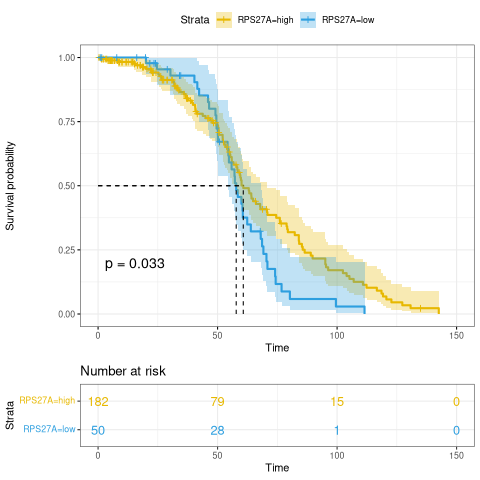
\includegraphics[width=0.7\linewidth]{figures/RPS27A.png}
			 	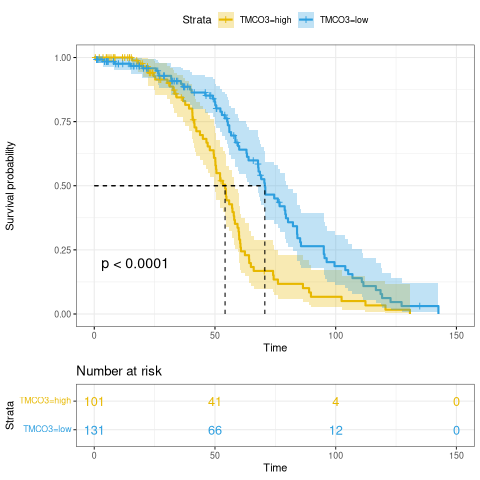
\includegraphics[width=0.7\linewidth]{figures/TMCO3.png}
	 			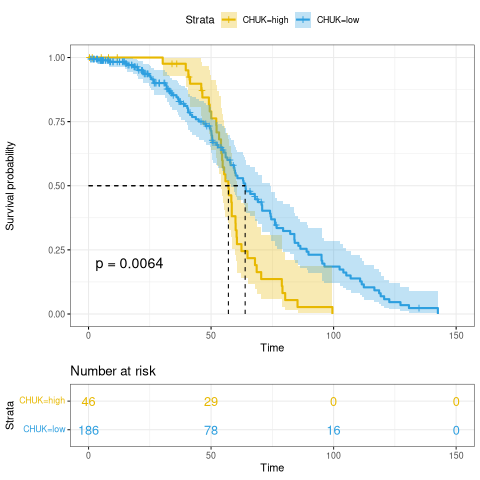
\includegraphics[width=0.7\linewidth]{figures/CHUK.png}
	 			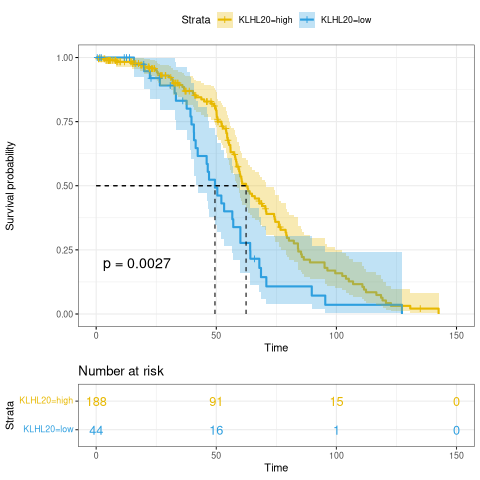
\includegraphics[width=0.7\linewidth]{figures/KLHL20.png}

				\columnbreak

		 		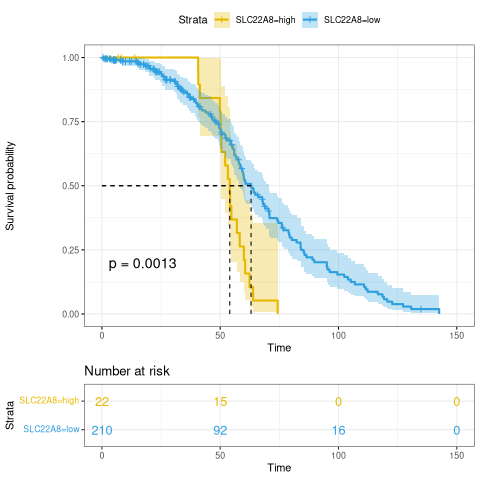
\includegraphics[width=0.7\linewidth]{figures/SLC22A8.png}
		 		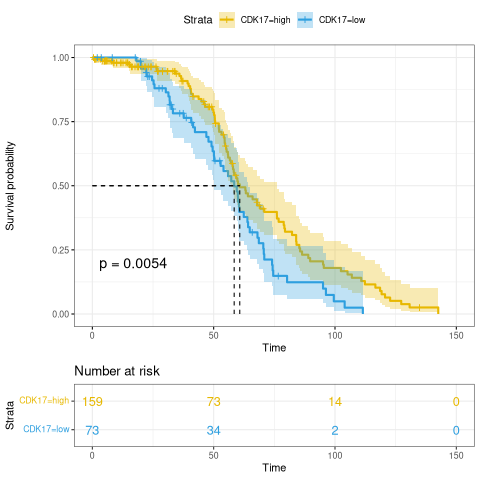
\includegraphics[width=0.7\linewidth]{figures/CDK17.png}
		 		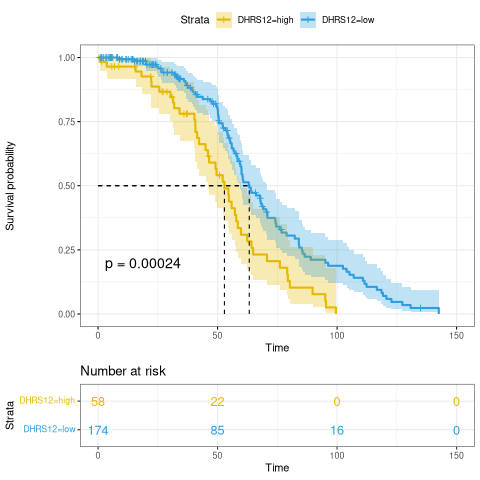
\includegraphics[width=0.7\linewidth]{figures/DHRS12.png}
		 		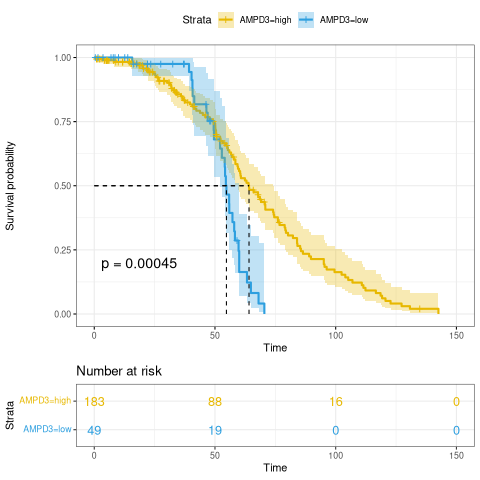
\includegraphics[width=0.7\linewidth]{figures/AMPD3.png}

			\end{multicols}
			\caption{Survival curves, on the left vitamin D related genes, on the right the top stage DEGs}
			\label{fig:surv_curve}
		 \end{figure*}

		For each of these gene the respective $HR$ can be found in table \ref{tab:hr}

		\begin{table}[ht]
			\begin{tabular}{|cc|cc|}
				\hline
				Vitamin D gene & HR & Stage DEG & HR\\
				\hline
				RPS27A & $1.4\cdot 10^8$ & SLC22A8 & $3.3\cdot 10^6$\\
				\hline
				TMCO3 & $7.9\cdot 10^5$ & CDK17 & $5.2\cdot 10^3$\\
				\hline
				CHUK & $88$ & DHRS12 & $2.9\cdot 10^3$\\
				\hline
				KLHL20 & $1.6\cdot 10^{-6}$ & AMPD3 & $2.6\cdot 10^{-7}$\\
				\hline
			\end{tabular}
			\caption{HR for significative genes}
			\label{tab:hr}
		\end{table}

\section{Discussion}
After having compiled the Kaplan-Meier curves the four genes derived from the consensus stage-based DEGs and the four gene found from the expanded vitamin D gene signature found statistically significant, we compiled a literature-based characterization for each of those (tables \ref{tab:vit_char} and \ref{tab:deg_char}.
\begin{table}[ht]
	\centering
	\small
	\begin{tabular}{cc}
		\hline
		Gene & Relevant function\\
		\hline
		RPS27A & \makecell{One of the genes encoding for ubiquitin.\\Misregulated in various cancers,\\including colorectal [n].\\Its upregulation in CRC\\may promote cancer cell proliferation\\and inhibition of apoptosis [o].}\\
		TMCO3 & \makecell{Probable Na(+) / H(+) antiporter.\\Linked to unfavorable outcomes in cancer [p].\\A patent exists for prognosis\\and treatment methods of\\CRC based on this gene [q].}\\
		CHUK & \makecell{Ser/Thr protein kinase involved in the\\(indirect) activation of NF-kB [f].\\Regulates cyclin D1. [g]\\Decreased activity is linked to cancer [h].}\\
		KLHL20 & \makecell{[i] Mediates ubiquitination of DAPK1\\thereby downregulating\\interferon-mediated apoptosis. [l]\\Mediates ubiquitination of PML thereby promoting\\resistance to hypoxia and cancer\\progression through HIF1a signalling. [m].}\\
		\hline
	\end{tabular}
	\caption{Statistically significant genes in the expanded vitamin-D gene signature}
	\label{tab:vit_char}
\end{table}

\begin{table}[ht]
	\small
	\centering
	\begin{tabular}{cc}
		\hline
		Gene & Relevant function\\
		\hline
		SLC22A8 & \makecell{Integral membrane protein involved in\\the sodium-dependent excretion of\\potentially toxic organic anions.\\Expression specific to kidney and brain [e].}\\
		CDK17 & \makecell{Cyclin-dependent protein \\serine/threonine kinase. Involved in the regulation \\of transcription involved in G1/S\\transition of mitotic cell cycle\\(source: GO biological process).\\Expressed in many tissues (no specificity) [b].\\It is the target of\\4 CDK inhibitors.}\\
		DHRS12 & \makecell{Oxidoreductase. Linked to poor prognosis\\in ovarian cancer [c] and\\suppression of proliferation\\and metastasis in osteosarcoma [d].}\\
		AMPD3 & \makecell{AMP deaminase in erythrocytes. In mice,\\mutations on this gene reduce levels\\of naive CD4+ and naive CD8+ cells\\in peripheral blood but not in lymphoid tissue.\\This is most likely due to a signalling\\mechanism triggered by the mutated\\phenotype of the red blood cells. [a].}\\
		\hline
	\end{tabular}
	\caption{4 top genes in stage DEGs}
	\label{tab:deg_char}
\end{table}




%----------------------------------------------------------------------------------------
%	REFERENCE LIST
%----------------------------------------------------------------------------------------
\phantomsection
\bibliographystyle{unsrt}
\bibliography{references}


\end{document}
